\documentclass[11pt]{article}
\usepackage[letterpaper, margin = 1 in]{geometry}
\usepackage{tabularx}
\usepackage{ltablex}
\usepackage{tabularray}
\usepackage{array}
\usepackage{booktabs}
\usepackage{longtable}
\usepackage{caption}
\usepackage{verbatim}
\usepackage{graphicx}
\usepackage{float}
\usepackage{xurl}


\title{\textbf{Revision 0: \\ System Design \\ \large Group 8 - C.A.V.E: Cave Assessment and Visualization Equipment}}
\author{Abdul Rahim Khan \\ Andrew Brink \\ Gokberk Yilmaz \\ Nicholas Trimble \\ Tabish Faisal}
\date{December 16, 2025}
\begin{document}
	\fussy
	\maketitle
	~\newpage
	\section{Introduction}
		The goal of this project is to create a portable device that can reliably and accurately reconstruct 3-D mappings of low light environments, such as crevice caves in the Niagara Escarpment, while avoiding the use of expensive technologies and solutions such as a 3-D LiDAR.
		\subsection{Purpose}
			This document will outline the specifications and design of the various modules within the device to achieve the requirements previously established. It will also partition these requirements into hardware and software sections and define the necessary interfaces and interactions between components. 
		\subsection{Scope}
			The entirety of the device’s design falls under the scope of this document, including the physical design, power delivery, data storage, and interactions between the portable recording device and the offline data processing algorithm. Hardware components will have their dimensions and electrical interfaces specified, and software components will be broken into modules to create well documented interfaces and hierarchical relationships. 
		\subsection{Context Diagrams}
\begin{figure}[H]
				\centering
				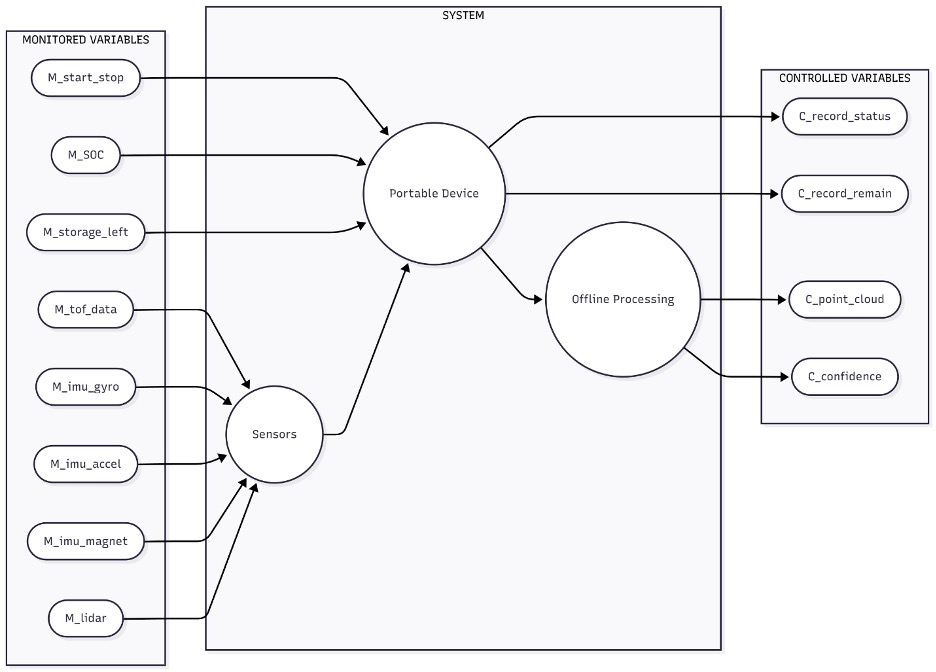
\includegraphics[width=0.9\textwidth]{images/SystemBoundaries.jpeg}
				\caption{Representation of System Boundaries}
				\label{fig:system}
			\end{figure}
		\subsection{Definitions}
			See System Requirements and Hazard Analysis section 2.1 for definitions relevant to this document. 
 % Nicholas' Section
	\section{System Hardware Components}

		\subsection{Raspberry Pi 5}
			A Raspberry Pi 5 single board computer (SBC) will be used for collecting and temporarily storing the information captured by the sensors of the system. 
		\subsubsection{Inputs and Outputs}
			Note that these are only within the context of the physical and electrical connections to the SBC. 
			\begin{tabularx}{\textwidth}{X X X p{0.45\textwidth}}
				\toprule
				\textbf{Direction} & 	\textbf{Name} & 	\textbf{Format} & 	\textbf{Description} \\
				\midrule
				Input & Start button & GPIO & User control over recording (\textit{M\_start\_stop}) \\
				Input & ToF Data & USB 2.0 & Series of point maps as captured by the time-of-flight sensor (M\_tof\_data) \\
				Input & IMU & I2C & Various orientation data (M\_imu\_gyro, M\_imu\_accel, M\_imu\_magnet) \\
				Input & 2D LiDAR & TBD  & Longer distance scans with a wider field-of-view (FOV) to aid in the point cloud merging (M\_lidar) \\
				Input & Power & USB-PD & 5V, 5A via the RPi Head board - \textit{Refer to Appendix A}. *Note that this is not USB-PD compliant \\
				Output & Capture Data & rosbag & Database of captured information from a recording session \\
				Output & Recording status & LED or button toggle & Indicates whether the a device is recording (C\_record\_status) \\
				Output & Remaining time & LEDs or display & Communicates recording time available to user (C\_record\_remain) \\
				\bottomrule
			\end{tabularx}

		\subsubsection{Behavior}
			Takes in power and the various sensor signals and routes them to the software running on the Pi’s system-on-chip. The software will provide appropriate outputs to control the sensors and drive the various GPIO. This component acheives requirement RE1. 
		\subsubsection{Dimensions}
\begin{figure}[H]
				\centering
				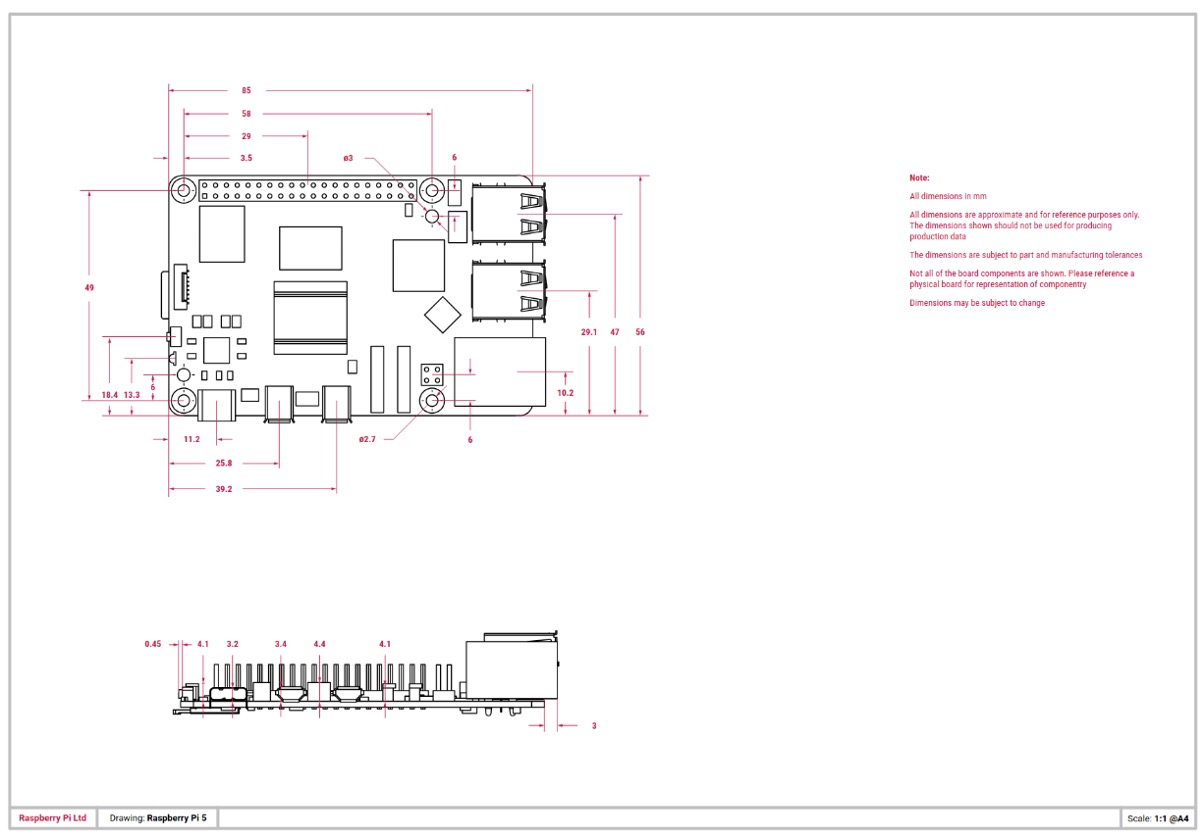
\includegraphics[width=0.9\textwidth]{images/RPi5.jpeg}
				\caption{Dimensions of Raspberry Pi 5}
				\label{fig:raspi5_D}
			\end{figure}
		\subsubsection{Electrical Interfaces}
			Refer to Raspberry Pi RP1 Peripherals in section 8 (References). 

	\subsection{ToF Sensor}
			The time-of-flight sensors used are SIPEED MaixSense A010 3D ToF sensors.
		\subsubsection{Inputs and Outputs}
			\begin{tabularx}{\textwidth}{X X X p{0.45\textwidth}}
				\toprule
				\textbf{Direction} & \textbf{Name} & \textbf{Format} & \textbf{Description} \\
				\midrule
				Input & Power & USB-C & 5V power from the Raspberry Pi \\
				Input & ToF Camera Captures & 940nm Laser & Depth information produced by the forward camera \\
				Output & ToF Data & USB 2.0 & 3D point cloud, continous scans (M\_tof\_data) \\
				\bottomrule
			\end{tabularx}
		\subsubsection{Behavior}
			This sensor measures the distance between itself and the environment around it and produces a series of point clouds representing a capture at a certain time instant. The interval between these captures is to be controlled by the data collection software subsystem (S1-M1) and will follow requirements RT1 and RT2.
		\subsubsection{Dimensions}
\begin{figure}[H]
				\centering
				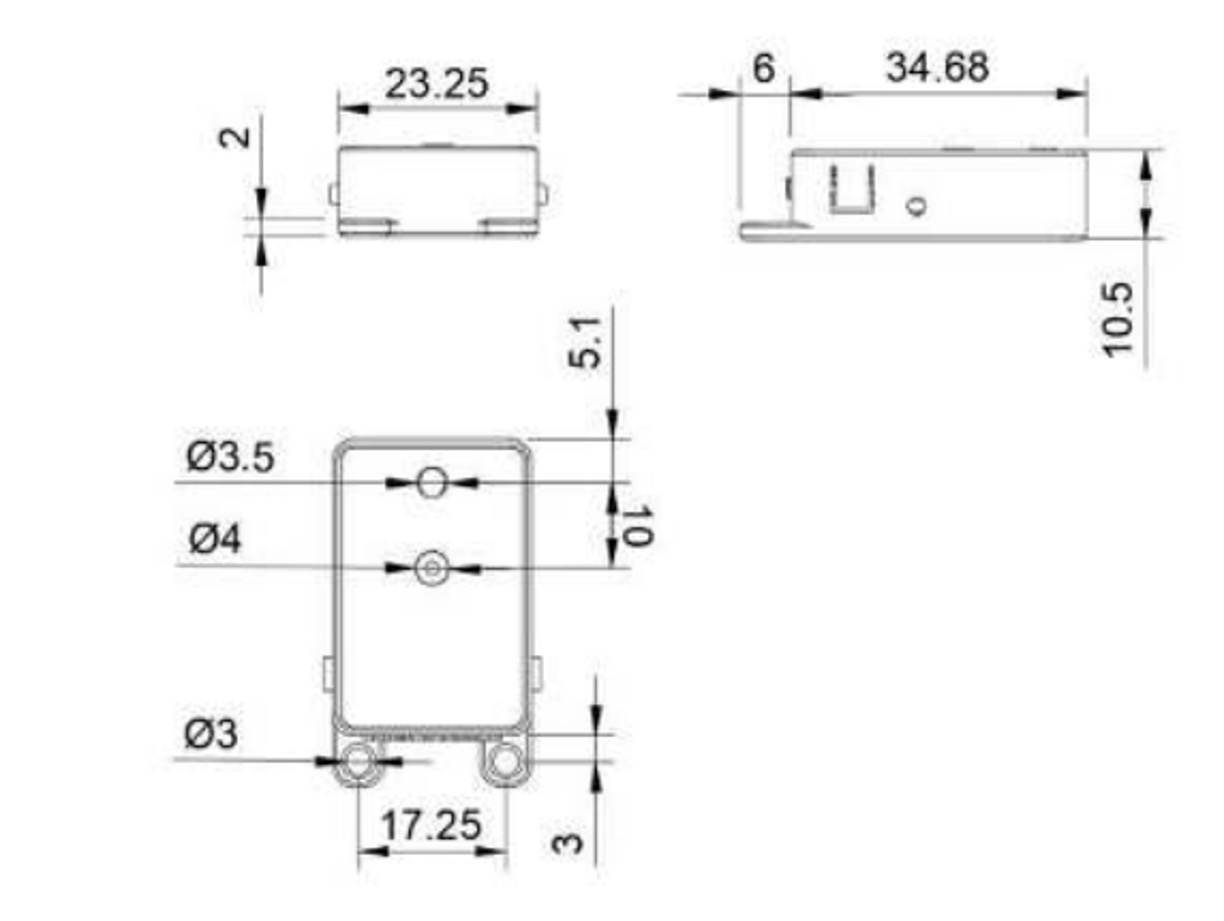
\includegraphics[width=0.9\textwidth]{images/ToF.jpeg}
				\caption{Dimensions of ToF sensor}
				\label{fig:ToF}
			\end{figure}
		\subsubsection{Electrical Interfaces}
\begin{figure}[H]
				\centering
				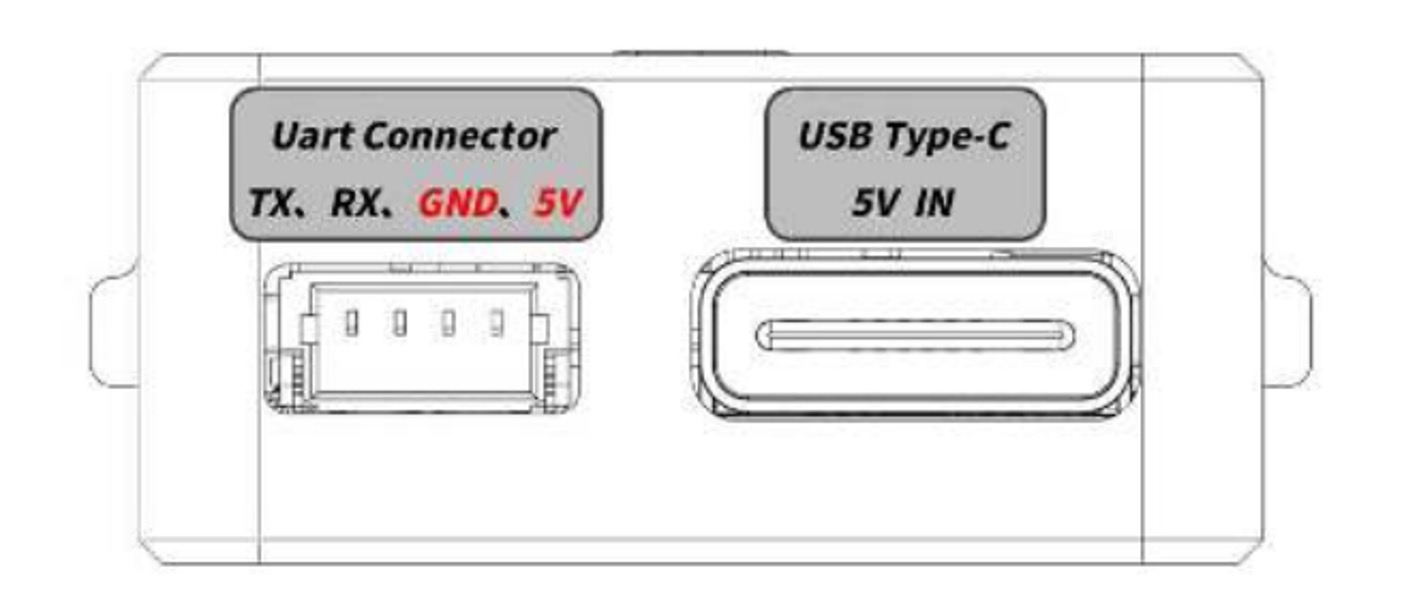
\includegraphics[width=0.9\textwidth]{images/ToF_EI.jpeg}
				\caption{Electrical Interfaces of ToF sensor}
				\label{fig:ToF_EI}
			\end{figure}
	\subsection{IMU}
		This component is the Adafruit BNO055 Absolute Orientation Sensor. 
		\subsubsection{Inputs and Outputs}
			\begin{tabularx}{\textwidth}{X X X p{0.45\textwidth}}
				\toprule
				\textbf{Direction} & \textbf{Name} & \textbf{Format} & \textbf{Description} \\
				\midrule
				Input & User Motion & Movement in 3D space & Movement of the operator through the scanning area \\
				Input & Power & 5V & Input power from the IMU connector \\
				Output & IMU data & I2C & Quaternion, linear acceleration, rotation, gravity, heading \\
				\bottomrule
			\end{tabularx}
		\subsubsection{Behavior}
			The IMU is a 9-axis sensor that will be used to determine displacement and rotation during scans. It produces fused data from a gyroscope, accelerometer, and geomagnetic sensor to produce matrices that represent displacements and rotations through the 3-D scanning area. Captures from this sensor will also be on an interval conforming to RT1 and RT2. 
		\subsubsection{Dimensions}
			Measurements in this figure are in inches.
\begin{figure}[H]
				\centering
				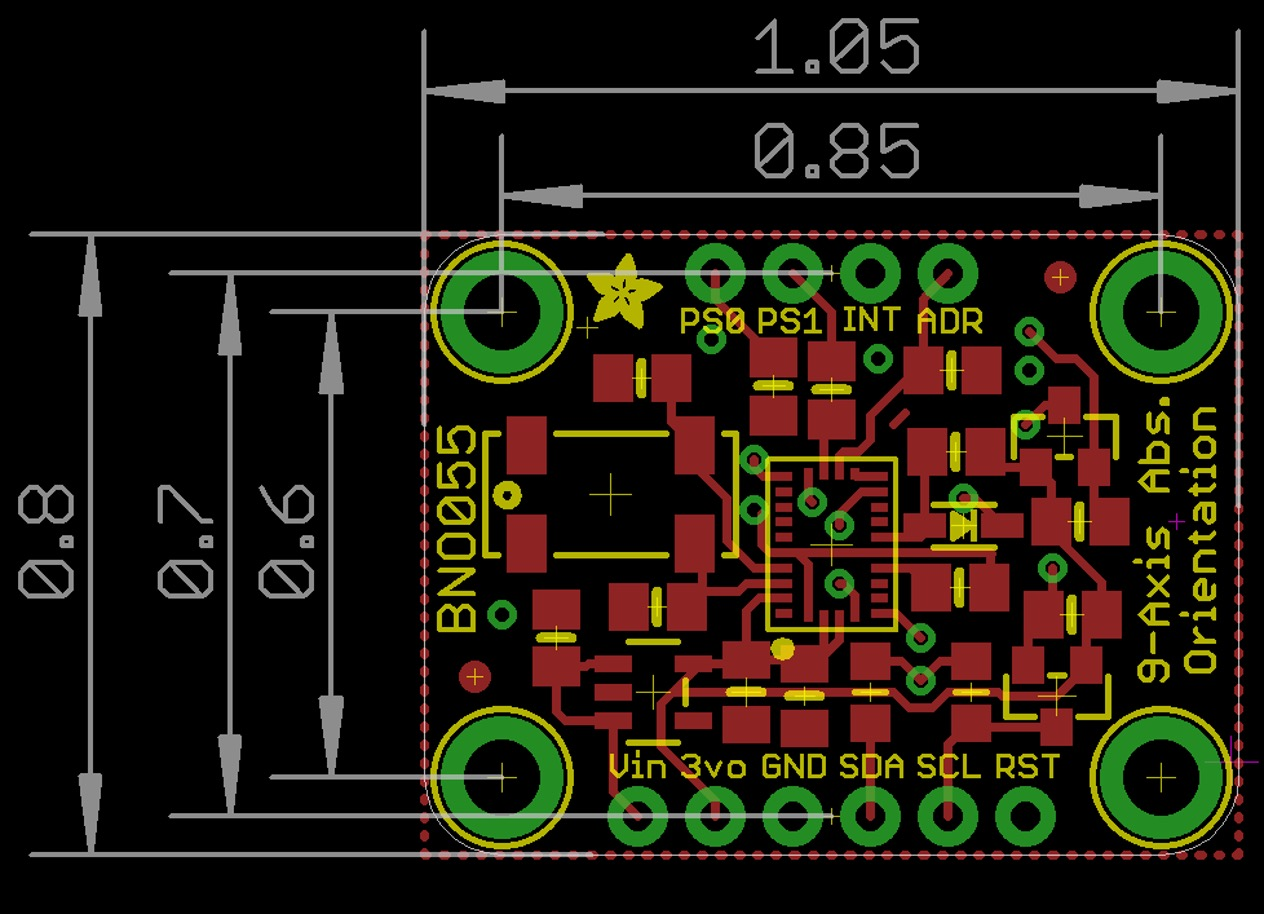
\includegraphics[width=0.9\textwidth]{images/IMU.jpeg}
				\caption{Dimensions of IMU}
				\label{fig:IMU}
			\end{figure}
		\subsubsection{Electrical Interfaces}
\begin{figure}[H]
				\centering
				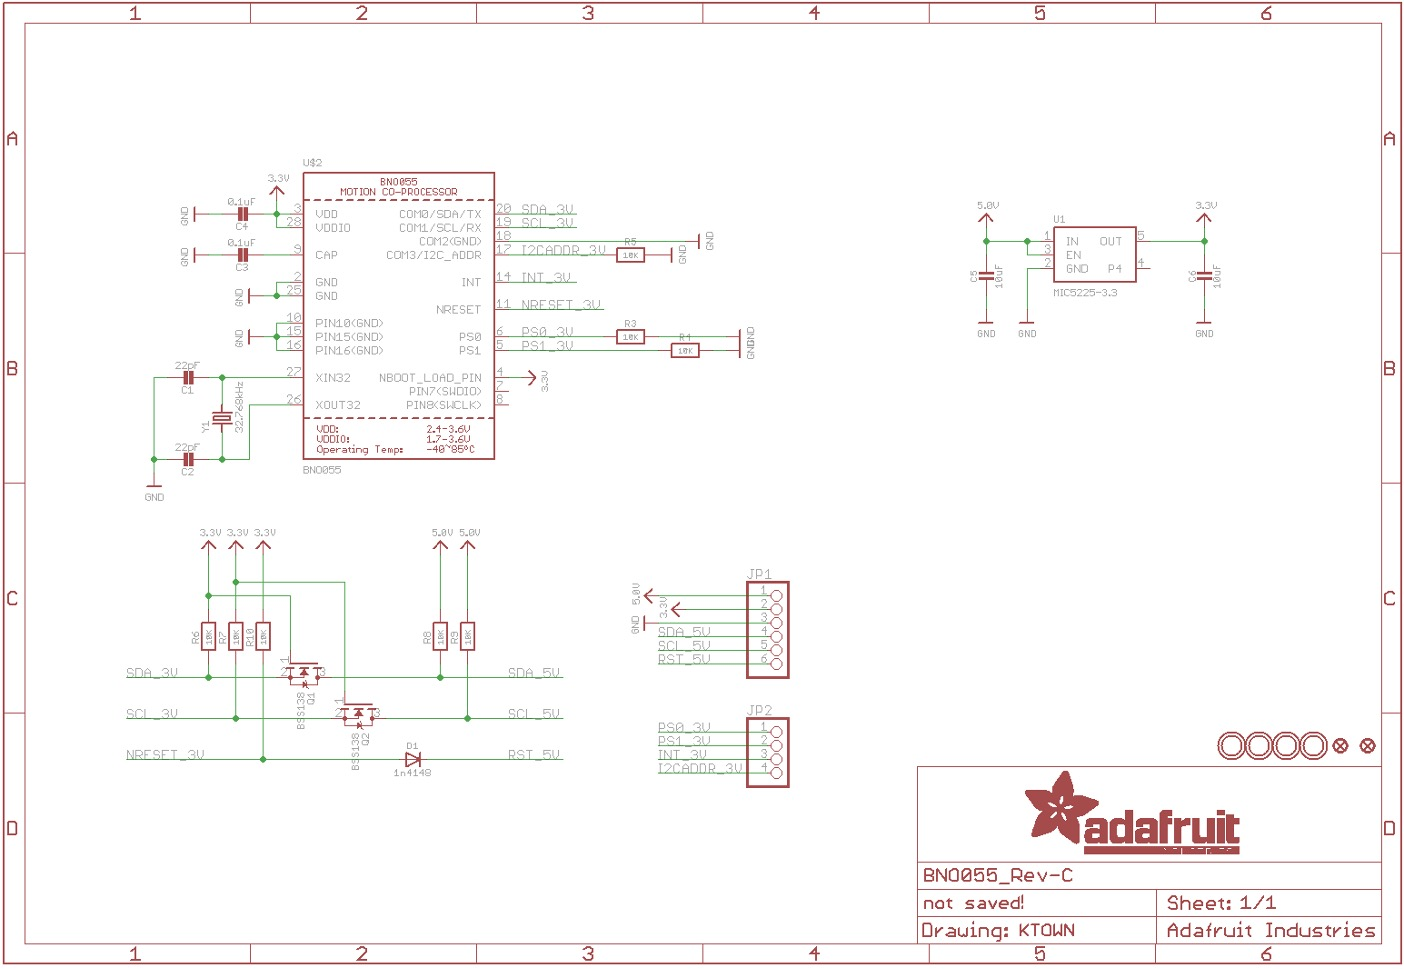
\includegraphics[width=0.9\textwidth]{images/IMU_EI.jpeg}
				\caption{Electrical Interfaces of IMU}
				\label{fig:IMU_EI}
			\end{figure}
	\subsection{2D Li-DAR}
		This component is available from Studica as the T-Mini LiDAR Kit. 
		\subsubsection{Inputs and Outputs}
			\begin{tabularx}{\textwidth}{X X X p{0.45\textwidth}}
				\toprule
				\textbf{Direction} & \textbf{Name} & \textbf{Format} & \textbf{Description} \\
				\midrule
				Input & Laser Scan & Point Cloud & 360 degree  scan of a single 2-D plane at 6-12Hz, 0.05-12m range \\
				Input & Power & 5V & Input power from the Raspberry Pi 5 \\
				Output & LiDAR scan & UART/USB & Digital output of each scan over either USB via a converter or directly through UART \\
				\bottomrule
			\end{tabularx}
		\subsubsection{Behavior}
			Scans a 2-D slice by rotating 360 degrees with a range of 0.05-12m and 0.54deg resolution. Provides an additional point cloud that will be used to help merge the more detailed 3-D scans from the ToF sensors, improving c\_confidence to conform to RB5. 
		\subsubsection{Dimensions}
			Measures 38.6mm wide and long, and 33.9mm tall, plus cable.
\begin{figure}[H]
				\centering
				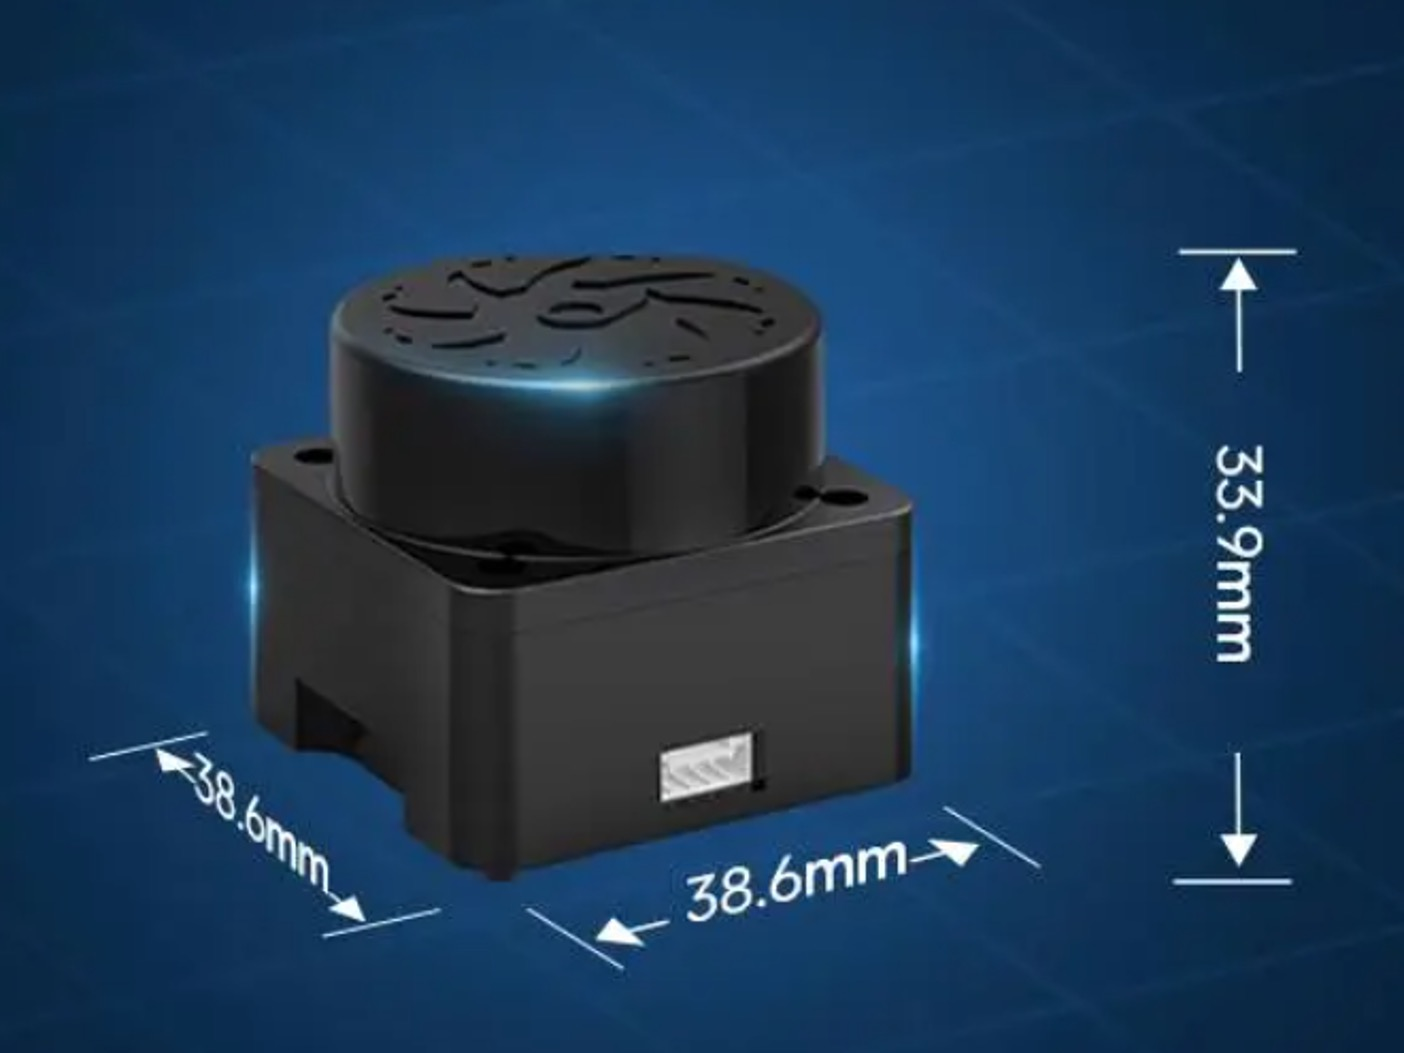
\includegraphics[width=0.9\textwidth]{images/2DLiDAR.jpeg}
				\caption{Dimensions of 2D-LiDAR}
				\label{fig:LiDAR}
			\end{figure}
		\subsubsection{Electrical Interfaces}
			Four pin JST-GH cable carrying 5V, UART Rx, UART Tx, and ground. 

	\subsection{Battery Pack}
		The exact pack used may change depending on price, availability, and depending on whether tests with lower input voltages (15V) prove feasible. Current designs are based on the UGREEN Nexode 100W 3-Port 20,000mAh power bank as it provides full 20V PD at a reasonable price and size. 
		\subsubsection{Inputs and Outputs}
			\begin{tabularx}{\textwidth}{X X X p{0.45\textwidth}}
				\toprule
				\textbf{Direction} & \textbf{Name} & \textbf{Format} & \textbf{Description} \\
				\midrule
				Input & Charging & USB-PD & Recharging of the battery pack from the wall in between scanning sessions \\
				Input & Power & USB-PD & Providing 20 or 15V power to the Rpi Head, then distributed to other devices \\
				\bottomrule
			\end{tabularx}
		\subsubsection{Behavior}
			This module is a standard USB-PD battery pack to provide safe, convenient, and portable power to the system. It will include a battery indicator to indicate to the user how much recording time is left and will be stored somewhere on the users’ person rather than on the helmet to lower to risk of it being damaged by low ceilings. Relevant requirements are RB4 and RE2.
		\subsubsection{Dimensions}
			It will fit in a pocket or small backpack, with this pack measuring 140mm high by 80mm wide by 30mm wide. 
		\subsubsection{Electrical Interfaces}
			Standard USB Type-C with at least USB 2.0 signalling to enable Power Delivery. 

	\subsection{Helmet Mount}
		\subsubsection{Inputs and Outputs}
			This module has no electrical signals or information to process and so has no inputs or outputs. From a mechanical standpoint its inputs are the masses of the TOF sensors, LiDAR, IMU, and Raspberry Pi, and its output is their combined masses loaded on the helmet. 
		\subsubsection{Behavior}
			The purpose of this module is to provide a stable surface for the helmet mounted components to be secured to a caving helmet. Each module must be in a position where it can carry out uninterrupted scans (ie. TOF facing outward, LiDAR has full 360 line of sight). To enable the custom shapes needed to hold various sizes of sensors on a round platform the material will likely be 3-D printed PLA plastic. This material provides sufficient strength for the relatively small and light sensors and allows heat-set inserts to securely screw the each component to it. The primary requirement to conform to is RE2.
		\subsubsection{Dimensions}
			Final dimensions of the module are to be determined but they must keep the mounted modules as close to the helmet as reasonable, so they should not exceed the approximate 400x300x200mm cube around the user’s head. 

	\section{Software Subsystem S1: Data Collection}

		\subsection{Module M1: Time-of-Flight (ToF) Sensor}
		\label{sec:M1}
			\subsubsection{Module Information}
				The ToF module is responsible for acquiring depth measurment data from the sensors and outputting time-stamped point cloud data. The module provides raw 3D point cloud frames in continuity that represents the surrounding environment. The hidden design decision in this module are the calibration parameters (i.e. serial access between sensor and the local system) and the calculation process from depth values to 3D point cloud maps. 
			\subsubsection{Uses Hierarchy}
			Uses: ROS2 Library/Module \\
			Used By: Module M5 (Data Aggregation)

			% Black-box -> What the module does, not how
			\subsubsection{MIS}
				The input and output of this module is given below:
				\begin{itemize}
					\item Input
						\begin{itemize}
							\item Raw ToF sensor measurements from environment capture (depth values and intensity with RGB color mapping)
						\end{itemize}
					\item Output
						\begin{itemize}
							\item Time-stamped point cloud frames
						\end{itemize}
				\end{itemize}
			% White-box -> enough detail to make coding trivial
			\subsubsection{MID}
				Methods:
				\begin{itemize}
					\item initialize\_tof
						\begin{itemize}
							\item Description: Establish serial connection from the ToF sensor to the connected system. 
							\item Parameters: None
							\item Returns: Status flag whether the sensor is detected or not. 
						\end{itemize}
					\item publish\_point\_cloud
						\begin{itemize}
							\item Description: Logs the calculated point cloud at a specified FPS. 
							\item Parameters: Depth-measurement data from ToF sensor
							\item Returns: Continuous point cloud frames at `x' FPS
						\end{itemize}
				\end{itemize}
			\subsubsection{Scheduling}
				The sensor data is read and publishes the point cloud frames in a set interval determined by the FPS value
			
		\subsection{Module M2: IMU}
		\label{sec:M2}
			\subsubsection{Module Information}
			The IMU provides inertial data to the Raspberry Pi, which will be used to improve the accuracy of our final model. This module reports the real-time rotation and acceleration data, which is logged for later use. 
			\subsubsection{Uses Hierarchy}
				Uses: None \\
				Used by: Module M3 (Data Aggregation)
			\subsubsection{MIS}
				\begin{itemize}
					\item Input:
						\begin{itemize}
							\item Analog inertial data from the environment
						\end{itemize}
					\item Output:
						\begin{itemize}
							\item Acceleration data, gyroscopic data, and linear acceleration data
						\end{itemize}
				\end{itemize}
			\subsubsection{MID}
				Methods:
				\begin{itemize}
					\item sensor\_acceleration
						\begin{itemize}
							\item Description: A getter function to read acceleration data form the BNO055 sensor over I2C 
							\item Parameters: None 
							\item Returns: Acceleration data
						\end{itemize}
					\item sensor\_gyro
						\begin{itemize}
							\item Description: A getter function to read gyroscopic data form the BNO055 sensor over I2C 
							\item Parameters: None 
							\item Returns: Gyroscope data
						\end{itemize}
					\item sensor\_linear\_acceleration
						\begin{itemize}
							\item Description: A getter function to read linear acceleration data form the BNO055 sensor over I2C 
							\item Parameters: None 
							\item Returns: Linear acceleration data
						\end{itemize}
				\end{itemize}
			\subsubsection{Scheduling}
				The sensor data needs to be read every time step, but can be logged to non-volatile storage at any point during operation. 
			\subsubsection{Initialization}
				The sensor is initialized over the I2C bus with the libraries provided by the manufacturer.  

		\subsection{Module M3: Data Aggregation}
		\label{sec:M3}
			\subsubsection{Module Information}
			The data aggregation module is responsible for producing time-aligned sensor data and synchronize each ToF point cloud frame with the IMU data to the closest time ($\Delta_{t\_IMU} - \Delta_{t\_point\_cloud}$) it was acquired. 
			\subsubsection{Uses Hierarchy}
				Uses: Module M1 (ToF sensor) and Module M2 (IMU)\\ 
				Used by: None
			\subsubsection{MIS}
				\begin{itemize}
					\item Inputs:
						\begin{itemize}
							\item Stream of ToF point cloud frames 
							\item Stream of IMU data 
						\end{itemize} 
					\item Outputs:
						\begin{itemize}
							\item Live data packet (ROS2 Node) containing time-matching point cloud and IMU data
						\end{itemize}
				\end{itemize}
			\subsubsection{MID}
				Methods:
				\begin{itemize}
					\item push\_cloud\_frame
						\begin{itemize}
							\item Description: Insert new point cloud frame into a buffer along with it's timestamp 
							\item Parameters: Timestamped point cloud frame
							\item Returns: Boolean (True for success)
						\end{itemize}
					\item push\_imu\_data
						\begin{itemize}
							\item Description: Insert new IMU data into an IMU buffer
							\item Parameters: Timestamped IMU data 
							\item Returns: Boolean (true for success)
						\end{itemize}
					
					\item sync\_data
							\begin{itemize}
								\item Description: Synchronizes the point cloud frame in buffer with the closest-time IMU data in the secondary  
								\item Parameters: None 
								\item Returns: Data packet containing matching point cloud frame and IMU data
							\end{itemize} 
					\item send\_data\_packet
						\begin{itemize}
							\item Description: Outputs the recently synchronized data packet and clears out the buffers
							\item Parameters: None
							\item Returns: Synchronized data packet
						\end{itemize}
				\end{itemize}
			\subsubsection{Scheduling}
				This module is triggered everytime a point cloud frame or IMU data is received
			%\subsubsection{Initialization}
		
		\subsection{Module M4: Rosbag Recorder}
			\subsubsection{Module Information}
				This module records the synchronized sensor data packet and stores it as a rosbag file so that it can be used later in the point cloud processing.
			\subsubsection{Uses Hierarchy}
				Uses: Module M3 (Data Aggregation) \\
				Used By: Module M5 (Data Ingest)
			\subsubsection{MIS}
				\begin{itemize}
					\item Input:
						\begin{itemize}
							\item Synchronized data packet
							\item Storage path 
						\end{itemize}
					\item Output:
						\begin{itemize}
							\item Rosbag file 
						\end{itemize}
				\end{itemize}
			\subsubsection{MID}
			Methods:
			\begin{itemize}
				\item start\_record
					\begin{itemize}
						\item Description: Starts recording the synchronized data packet stream
						\item Parameters: Data packet
						\item Returns: Rosbag file containing continuous data packets
					\end{itemize}
				\item check\_rosbag\_directory
					\begin{itemize}
						\item Description: Checks whether directory/file exists for storing the rosbag file
						\item Parameters: Path to directory/file
						\item Returns: Boolean (0 if directory/file does not exist)
					\end{itemize}
			\end{itemize}
			\subsubsection{Scheduling}
				Starts upon user input
	\section{Software Subsystem S2: Point Cloud Processing}

		\subsection{Module M5: Data Ingest}
		\label{sec:M4}
			\subsubsection{Module Information}
				The Data Ingest module is part of the Point Cloud Processing subsystem. The responsibility of this module is to take the data previously collected by the Data Collection subsystem, which is stored in the form of a rosbag, and prepare it for use by the other modules in this subsystem. 
			\subsubsection{Uses Hierarchy}
				Uses: Module M4 (Rosbag Recorder)\\
				Used by: Module M6 (Sensor Fusion) 
			\subsubsection{MIS}
				\begin{itemize}
					\item Input:
						\begin{itemize}
							\item Rosbag file
						\end{itemize} 
					\item Outputs:
						\begin{itemize}
							\item IMU messages 
							\item Data from ToF sensors 
							\item Data from 2D LiDAR sensor, if applicable
						\end{itemize}
				\end{itemize}
			\subsubsection{MID}
Methods 
\begin{itemize}
\item set\_rosbag\_filename 
	\begin{itemize}
\item Description: Attempt to access file specified 
\item Parameters: String representing filename 
\item Returns: True if rosbag is valid 
	\end{itemize}
\item get\_imu\_message 
	\begin{itemize}
\item Parameters: none 
\item Return: IMU data at a specific instant in time and timestamp, or indication of failure if no data is available. 
	\end{itemize}
\item get\_tof\_frame 
	\begin{itemize}
\item Parameters: index of tof camera to access 
\item Return: Depth image (or point cloud) of data recorded by specified ToF camera with timestamp, or indication of failure if no data is available. 
	\end{itemize}
\item get\_lidar\_frame 
	\begin{itemize}
\item Parameters: none 
\item Return: Point cloud of data captured by LiDAR with timestamp, or indication of failure if no data is available. 
	\end{itemize}
\end{itemize}
			\subsubsection{Scheduling}
			There are no scheduling requirements, as this subsystem does not operate in real time. The functions may be called whenever the other modules are ready for the data. 
			%\subsubsection{Initialization}


		\subsection{Module M6: Sensor Fusion}
			\subsubsection{Module Information}
			This module uses the data from the IMU, ToF, and LiDAR sensors to build a 3D point cloud. The IMU data is integrated to provide an initial estimate of the transformation between two ToF captures. This estimate is used to perform point cloud alignment for each new point cloud produced by the ToF cameras. Finally, the LiDAR data is added to the point cloud, to increase the range. 
			\subsubsection{Uses Hierarchy}
				Uses: Module M5 (Data Ingest)\\
				Used by: None 
			\subsubsection{MIS}    
			\begin{itemize}
		\item Inputs 
			\begin{itemize}
		\item IMU data 
		\item ToF data 
		\item LiDAR data 
			\end{itemize}
		\item Outputs 
			\begin{itemize}
		\item 3D point cloud 
			\end{itemize}
			\end{itemize}

Methods 
\begin{itemize}
\item update\_imu 
	\begin{itemize}
		\item Description: Integrates new IMU data to estimate transformation 
		\item Input: imu data 
		\item Output: transformation from previous update\_tof time till now 
	\end{itemize}
\item update\_tof
	\begin{itemize}
\item Description: Using transformation estimated by IMU as initial guess, align point clouds 
\item Input: new point cloud that needs to be registered 
\item Output: transformation from previous point cloud to new point cloud 
	\end{itemize}
\item combine\_tof 
	\begin{itemize}
\item Description: Combines point clouds from the two tof sensor, so that they can be treated as one for update\_tof step 
\item Input: two different point clouds with same timestamp from separate cameras 
\item Output: one point cloud 
	\end{itemize}
\item update\_lidar 
	\begin{itemize}
\item Description: Add points measured by LiDAR sensor to full point cloud data member 
\item Input: point cloud from LiDAR (2D) 
	\end{itemize}
\item get\_point\_cloud 
	\begin{itemize}
\item Description: Get the full point cloud with all data that has been processed so far 
\item Output: full point cloud. 
	\end{itemize}
\end{itemize}
			\subsubsection{MID}
Private data members 
\begin{itemize}
	\item point\_cloud $\rightarrow$ Collection of points in 3D space which represent all the data that has been processed so far 
	\item imu\_state $\rightarrow$ Pose (position and orientation) of IMU, with 1st and 2nd derivatives (velocity and acceleration), to be updated by Kalman filter 
	\item imu\_state\_covariance $\rightarrow$ Covariance matrix corresponding to imu\_state, used by Kalman filter. 
	\item tof\_transforms $\rightarrow$ List or key-value structure containing timestamps and transformations as calculated by update\_tof 
\end{itemize}
Design of methods 
\begin{itemize}
\item update\_imu $\rightarrow$ A Kalman Filter (or a variation such as the Error State Kalman filter) is used to predict the movement of the helmet, using acceleration, gyroscope, and magnetometer data. 
\item update\_tof $\rightarrow$ Use Iterative Closest Point (ICP) algorithm, using an implementation such as that in Point Cloud Library (PCL), to find the transformation between the previous ToF sensor point cloud and the new one. This transformation, together with the timestamp, is stored in tof\_transforms. The estimate of the transformation which has been obtained using update\_imu is used as the initial guess for the ICP algorithm. 
\item combine\_tof $\rightarrow$ If the two point clouds have the same timestamp, append the points from one point cloud to the other point cloud. 
\item update\_lidar $\rightarrow$ Add the LiDAR points to point\_cloud, using the transformation matrix that has been calculated for the current timestamp from the update\_tof method. The use of ICP is not required or helpful here, because the points are from a 2D slice which is moving through space in 3D. 
\item get\_point\_cloud $\rightarrow$ Returns copy of point\_cloud private data member 
\end{itemize}

\subsubsection{Notes} 

\textit{The paper “Perception in the Dark” has been used as reference for how the Error State Kalman filter and ToF ICP can be implemented, and their open-source code will be used as a reference as well. This work is limited to one ToF sensor, however, and does not use 2D lidar.  (not sure how to cite this properly but here is a link: https://doi.org/10.3390/s20051263)}
			%\subsubsection{Scheduling}
			%\subsubsection{Initialization}

	\section{Normal Operation}
		The normal operation would include the following steps: 
		\begin{itemize}
			\item Power the system on 
			\item Allow ample time for required start-up sequences  \item There will be an indication as to when scanning begins 
			\item Scanning will continue until you manually stop it 
			\item Once scanning ends, it will process and produce the 3-D image of the scan  
			\item After we are done using the system, we may choose to either do another scan, or to turn off the system. 
		\end{itemize}
	\section{Undesired Event Handling}
		Undesired events can occur at each major step and in between them, 
		\begin{itemize}
			\item During turning the system on: 
			\begin{itemize}
				\item The system may not turn on 
				\begin{itemize}
					\item Related Hazards: “Battery capacity runs out”, H2R7, H2R8, H2R9
					\item In this case, we’d check if we properly turned it on,  
					\item If that does not work, we’d check if the battery is charged 
					\item If it still does not work, then we’d check any wiring 
				\end{itemize}
				\item The system may turn on but then crash/turn off 
					\begin{itemize}
						\item Related Hazards: H2R13, H2R14, H2R15, H2R29, H2R30
						\item In this case, this may be a software or sensor issue, in which case we’d have to determine the root cause. 
					\end{itemize}
			\end{itemize}
			\item While we wait for the start-up sequences 
			\begin{itemize}
				\item Previous iterations may try to start up again 
				\begin{itemize}
					\item Related Hazards: H2R11 
					\item Make sure all instances are closed during shut-down so that it wouldn’t restart 
				\end{itemize}
			\item Specific parts may fail or have an error 
				\begin{itemize}
					\item Related Hazards: All hazards can fall under this umbrella. 
					\item Using well-defined error/loading messages to determine which part of the system particularly is giving issues, and work on countermeasures accordingly 
				\end{itemize}
			\item The battery may suddenly run out 
				\begin{itemize}
					\item Related Hazards: “Battery Issue” 
					\item If this happens, ensure proper shutdown protocol so even if it suddenly loses power, it wouldn’t have devastating consequences 
				\end{itemize}
			\end{itemize}
			\item When the scanning begins, 
			\begin{itemize}
				\item The battery may run out during scanning 
				\begin{itemize}
					\item Related Hazards: “Battery Issue” 
					\item Since the scan is stored in RAM, the ongoing scan will be lost, however  
				\end{itemize}
				\item The indicator doesn’t indicate correctly 
					\begin{itemize}
						\item Related Hazards: H2R7 H2R8 H2R9 H2R11 
						\item Have a second indicator just in case $\rightarrow$ if this fails, then have to check the entire system 
						\item Ensure it isn't a human error, if not then have to check the system for the fault
					\end{itemize}
				\item Sudden/erratic movement for scanning 
					\begin{itemize}
						\item Related Hazards: H2R20, H2R22, H2R23 
						\item Correct training on handling. 
						\item Try and handle it by having “blank” space instead of warped space. 
						\item Well timed snapshots to ensure minimal loss/warping.
						\item In extreme cases, erasure of the entire scan. 
					\end{itemize}
			\end{itemize}
			\item When scanning ends, 
			\begin{itemize}
				\item Manual stopping may not work
					\begin{itemize}
						\item Related Hazards: H2R7, H2R8, H2R9, H2R11 
						\item Have a secondary method to manually stop the scan. 
						\item Allow scans to save dynamically if there is a sudden shut-down, allowing us to in extreme cases disconnect whilst retaining information . 
					\end{itemize}
				\item Automatic stopping may not work 
					\begin{itemize}
						\item Related Hazards: H2R11 
						\item Have a visual indicator for time left in the scanner, to ensure it was supposed to stop. 
						\item Override automatic stopping with manual stopping.
					\end{itemize}
				\item Scan may be lost
					\begin{itemize}
						\item Related Hazards: H2R11 
						\item Store the frames dynamically in such a way where when a sudden issue occurs, it will keep it safe. 
						\item Have backup/concurrent instances saved in case one fails. 
					\end{itemize}
				\item Battery runs out 
					\begin{itemize}
						\item Related Hazards: “Battery Issue” 
						\item Make sure most progress won’t be lost. It is okay if the algorithm breaks suddenly, but it shouldn’t affect the frames
					\end{itemize}
			\end{itemize}
			\item Producing the 3-D image of the scan, 
			\begin{itemize}
				\item Battery runs out
					\begin{itemize}
						\item Related Hazards: “Battery Issue” 
						\item Have a buffer of raw processed files so that it can reproduce the image if needed.  
					\end{itemize}
			\end{itemize}
			\item When it comes to repeating the scan or turning off, 
			\begin{itemize}
				\item Doesn’t turn off
					\begin{itemize}
						\item Related Hazards: H2R11 
						\item Allow a secondary override to forcefully shut down the system without catastrophic failure. 
					\end{itemize}
				\item The repeat uses the same data as before
					\begin{itemize}
						\item Related Hazards: H2R11 
						\item Make sure shared variables are proper initialized and set to the default value before starting up. 
						\item This can be done through double-checking via validation.  
					\end{itemize}
			\end{itemize}
		\end{itemize}
	\newpage
	\section{Appendix A: Sandmaze PCBs}
		Last years’ Sandmaze group created several PCBs which this group will build off to better integrate the data collection subsystem. 

		\subsection{Rpi Head} 
			\subsubsection{Inputs and Outputs}
			\begin{tabularx}{\textwidth}{X X X p{0.45\textwidth}}
				\toprule
				\textbf{Direction} & 	\textbf{Name} & 	\textbf{Format} & 	\textbf{Description} \\
				\midrule
				Input & Start button & USB Type-C & Power and data connection to the IMU \\
				Input & ToF Data & USB 2.0 & Series of point maps as captured by the time-of-flight sensor (M\_tof\_data) \\
				Input & PD Input & USB-PD & Standard 20V USB PD sink \\
				Input & User Buttons  & SMT side mounted buttons (U6/8) & Allows user actuation of GPIO pins- pull down connection \\
				Output & RPi GPIO & 2x20 pin 2.54mm pitch header & IMU and button connections to Raspberry Pi SBC \\
				Output & Pi Power & USB Type-C & 5V5A power for RPi5, connecting to ‘Fake Wire’ \\
				Output & User LEDs & SMT LEDs & Display status of power conversion, some connected to GPIO (LED1/2, U10) \\
				\bottomrule
			\end{tabularx}



			\subsubsection{Behaviour}

This board connects on top of the Raspberry Pi 5 as a ‘hat’ device to break out some of the GPIO pins into more useful forms and provide power from the battery. The most important function it performs is to buck-convert the standard USB-PD power from the battery pack into the non-standard 5V5A supply required by the Pi 5 to avoid voltage drops in high load scenarios. The USB-PD spec only allows up to 3A to be supplied at 5V profiles, necessitating this conversion. It also provides a connection for the IMU Connector’s USB Type-C cable which is then attached to the I2C GPIO pins. There are also buttons and LEDs attached to GPIO pins. 

\subsubsection{Dimensions}

The board is the same dimensions as a Raspberry Pi (see section 2.1), with mounting holes in the same positions to allow it to be securely stacked on top of the Pi. 

\begin{figure}[H]
				\centering
				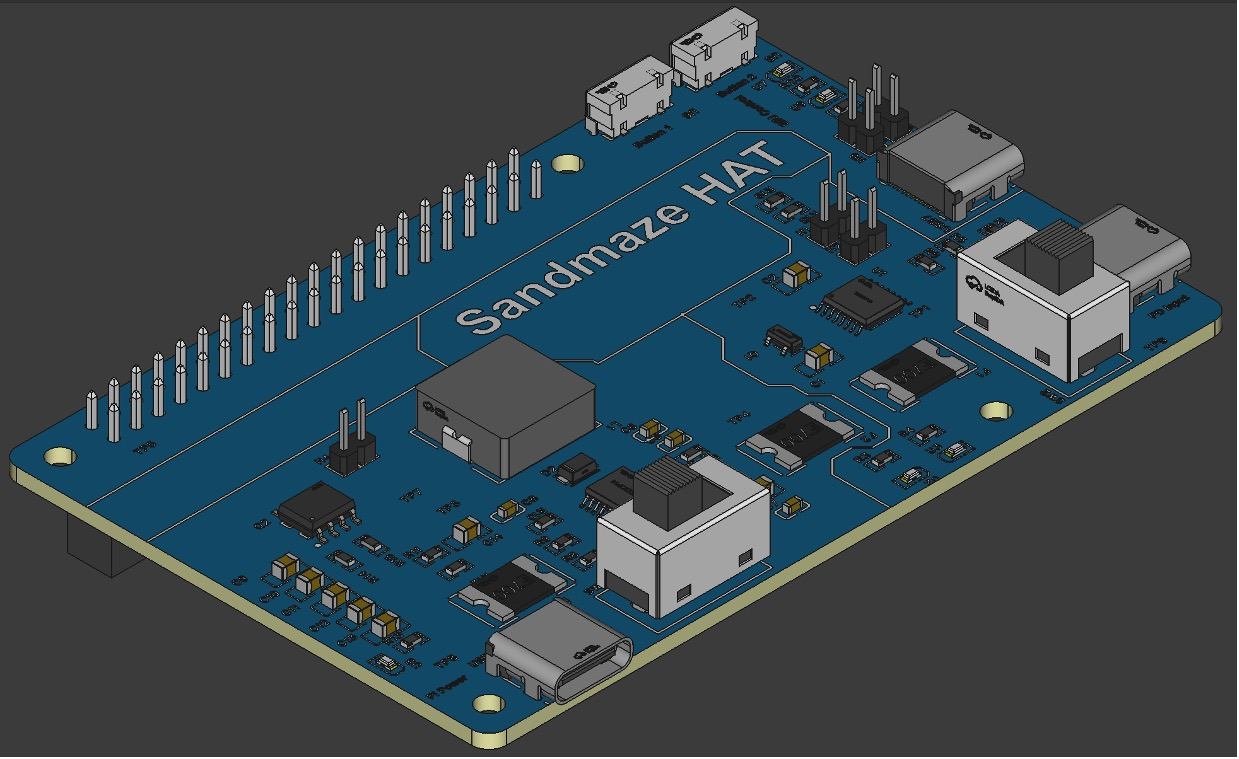
\includegraphics[width=0.9\textwidth]{images/Sandmaze.jpeg}
			\caption{Dimensions of Sandmaze HAT}
				\label{fig:Sandmaze}
			\end{figure}

\subsubsection{Electrical Interfaces}


\begin{figure}[H]
				\centering
				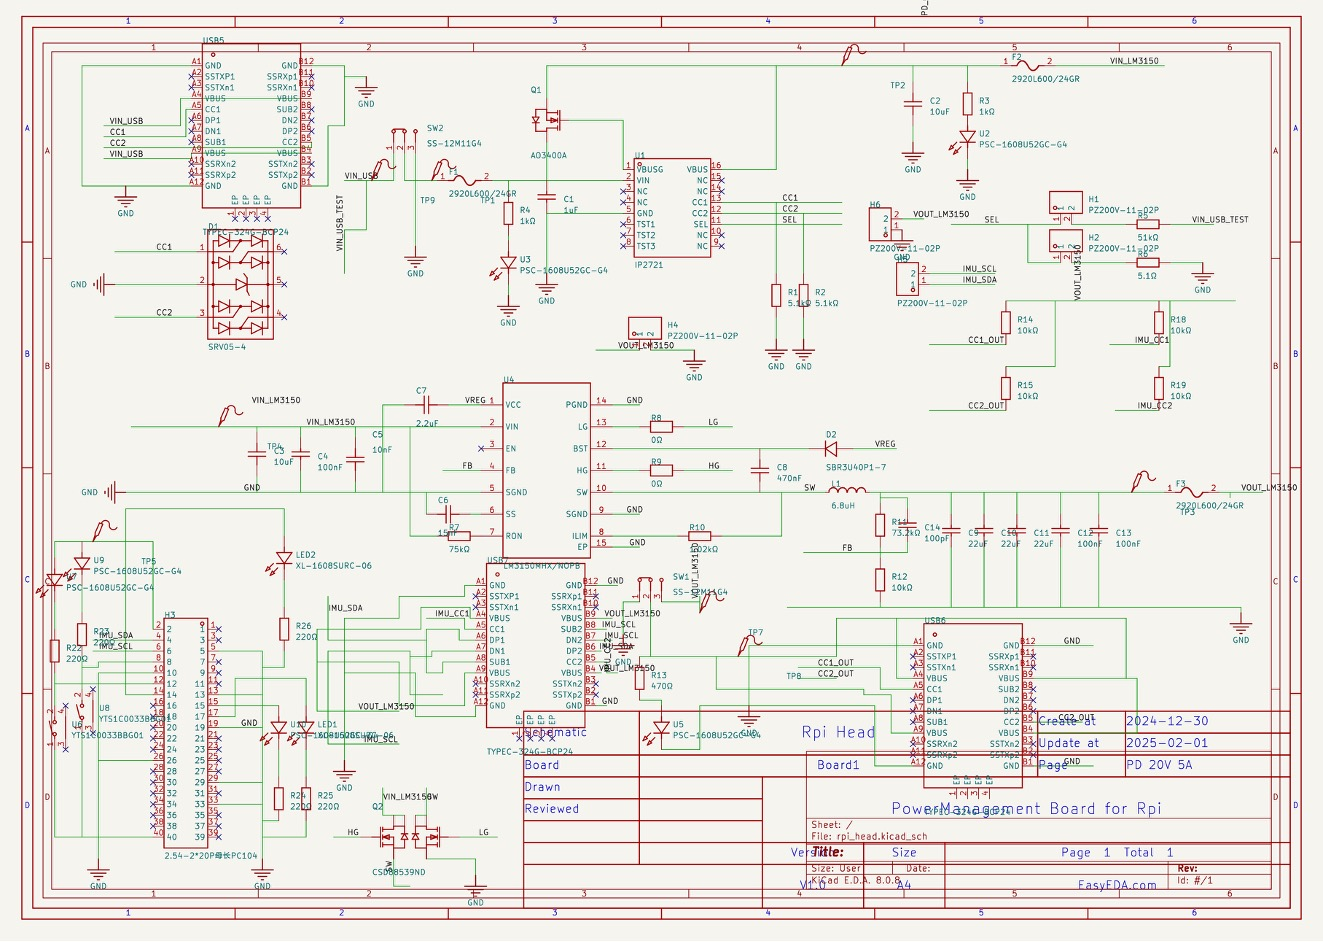
\includegraphics[width=0.9\textwidth]{images/Sandmaze_EI.jpeg}
			\caption{Electrical Interfaces of Sandmaze HAT}
				\label{fig:Sandmaze_EI}
			\end{figure}

\subsection{IMU Connector}

\subsubsection{Inputs and Outputs}

			\begin{tabularx}{\textwidth}{X X X p{0.45\textwidth}}
				\toprule
				\textbf{Direction} & 	\textbf{Name} & 	\textbf{Format} & 	\textbf{Description} \\
				\midrule
				Input & IMU header & 2.54mm header pins & Power and data connection to the IMU \\
				Output & IMU USB & USB Type-C & IMU wires re-pinned to use Type-C \\
				\bottomrule
			\end{tabularx}



			\subsubsection{Behaviour}

This board passes through the connections from the IMU board, converting the connector from a 1x6 pin 2.54mm pitch pin header to a standard USB Type-C connector. 

\subsubsection{Dimensions}
\begin{figure}[H]
				\centering
				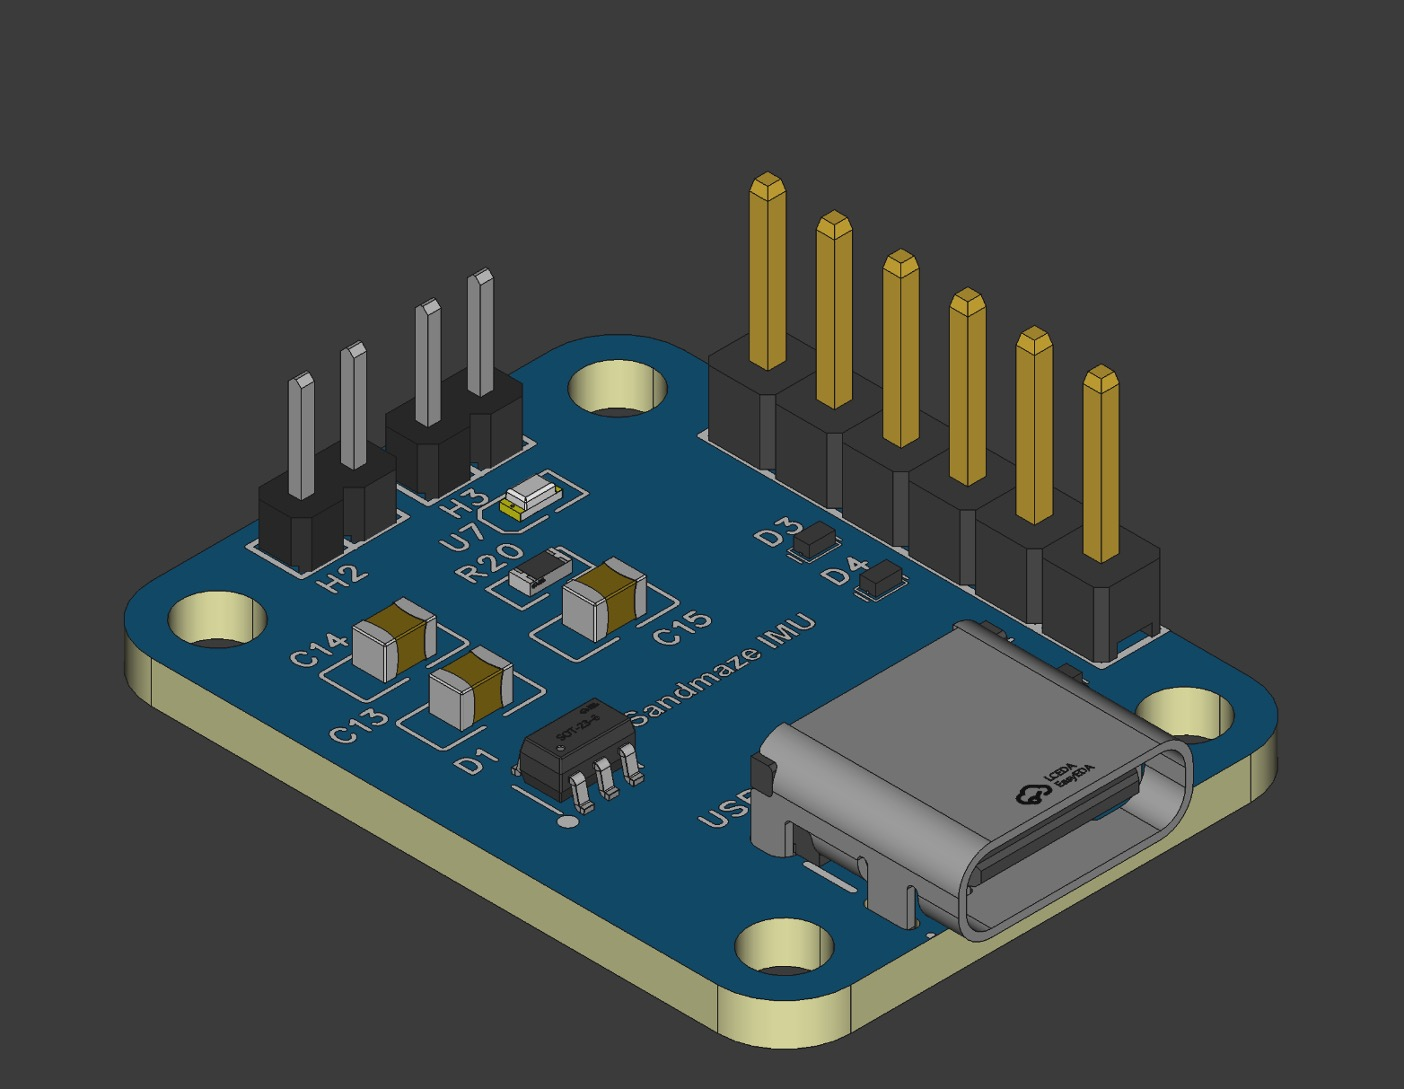
\includegraphics[width=0.9\textwidth]{images/IMU_connector.jpeg}
				\caption{Dimensions of IMU connector}
				\label{fig:IMU_connector}
			\end{figure}


\subsubsection{Electrical Interfaces}

\begin{figure}[H]
				\centering
				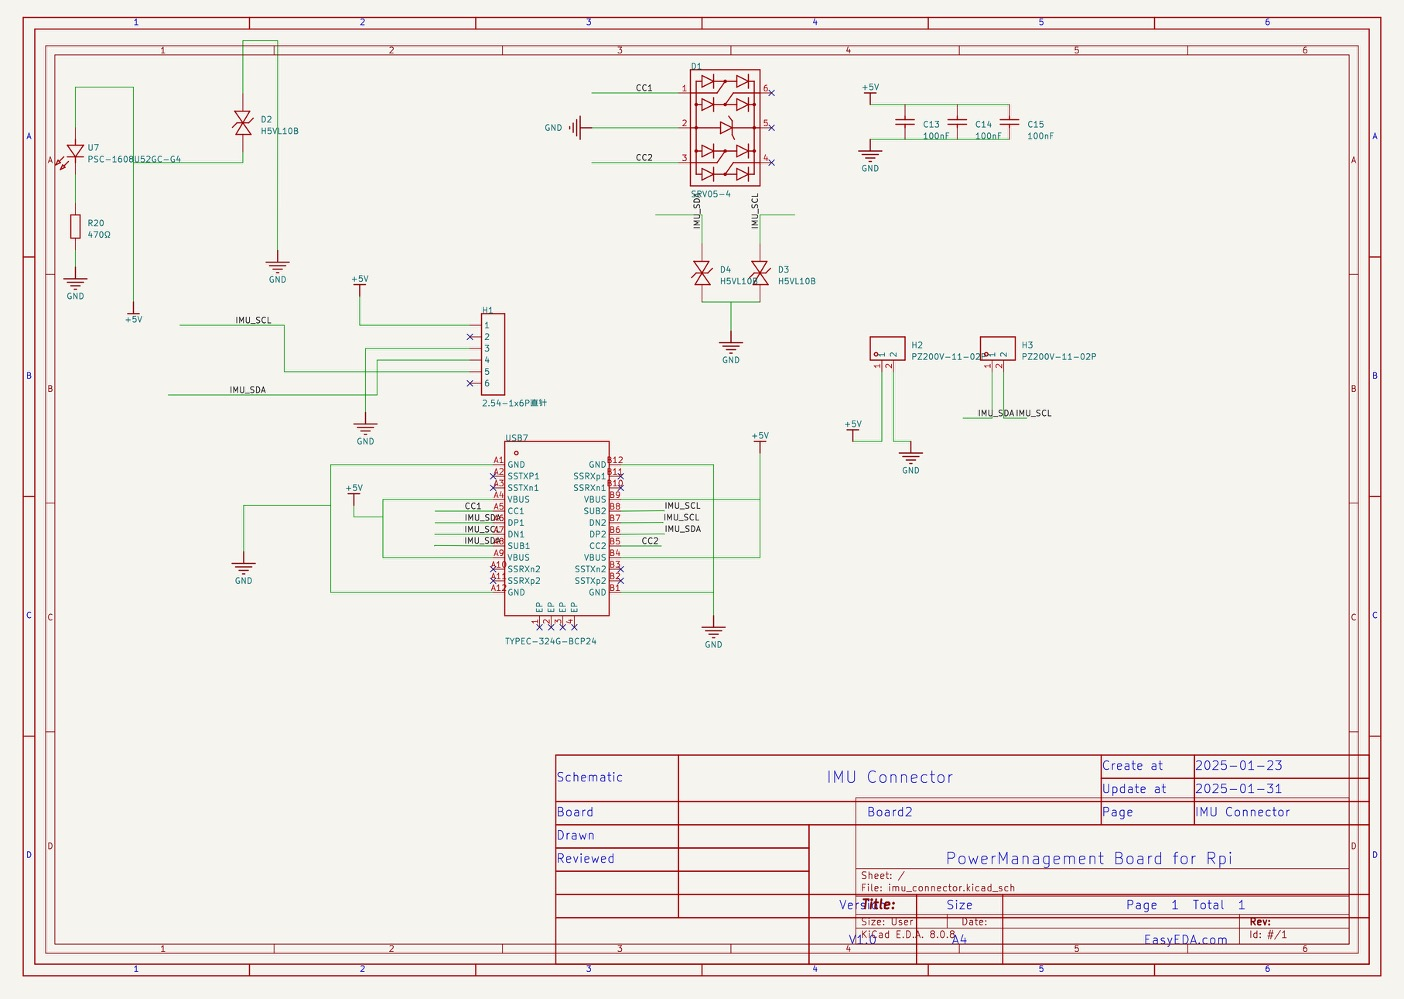
\includegraphics[width=0.9\textwidth]{images/IMU_connector_EI.jpeg}
			\caption{Electrical Interfaces of IMU connector}
				\label{fig:IMU_connectori_EI}
			\end{figure}
			\begin{tabularx}{\textwidth}{X X X X}
				\toprule
				\textbf{Pin} & \textbf{Purpose} & \textbf{Pin} & \textbf{Purpose} \\
				\midrule
				H1-1 & 5V to IMU & USB7-VBUS & 5V from Pi \\
				H1-3 & GND for IMU & USB7-GND & GND to Pi \\
				H1-4 & IMU SDA & USB7-DN* & IMU SCL \\
				H1-5 & IMU SDL & USB7-DP* & IMU SDA \\
				\bottomrule
			\end{tabularx}


			\begin{tabularx}{\textwidth}{X X X p{0.45\textwidth}}
				\toprule
				\textbf{Direction} & 	\textbf{Name} & 	\textbf{Format} & 	\textbf{Description} \\
				\midrule
				Input & IMU header & 2.54mm header pins & Power and data connection to the IMU \\
				Output & IMU USB & USB Type-C & IMU wires re-pinned to use Type-C \\
				\bottomrule
			\end{tabularx}
			\subsection{‘Fake Wire’ USB Type-C extension }

			\subsubsection{Inputs and Outputs}

			\begin{tabularx}{\textwidth}{X X X p{0.45\textwidth}}
				\toprule
				\textbf{Direction} & 	\textbf{Name} & 	\textbf{Format} & 	\textbf{Description} \\
				\midrule
				Input & RPi Head power  & USB Type-C & 5V5A power from the RPi Head \\
				Output & RPi5 Power & USB Type-C & 5V5A power to the Raspberry Pi 5 \\
				\bottomrule
			\end{tabularx}




			\subsubsection{Behaviour}

This is a pure passthrough acting as a short cable between the RPi Head’s power output port and the power input on the Raspberry Pi 5. 

\subsubsection{Dimensions}

\begin{figure}[H]
				\centering
				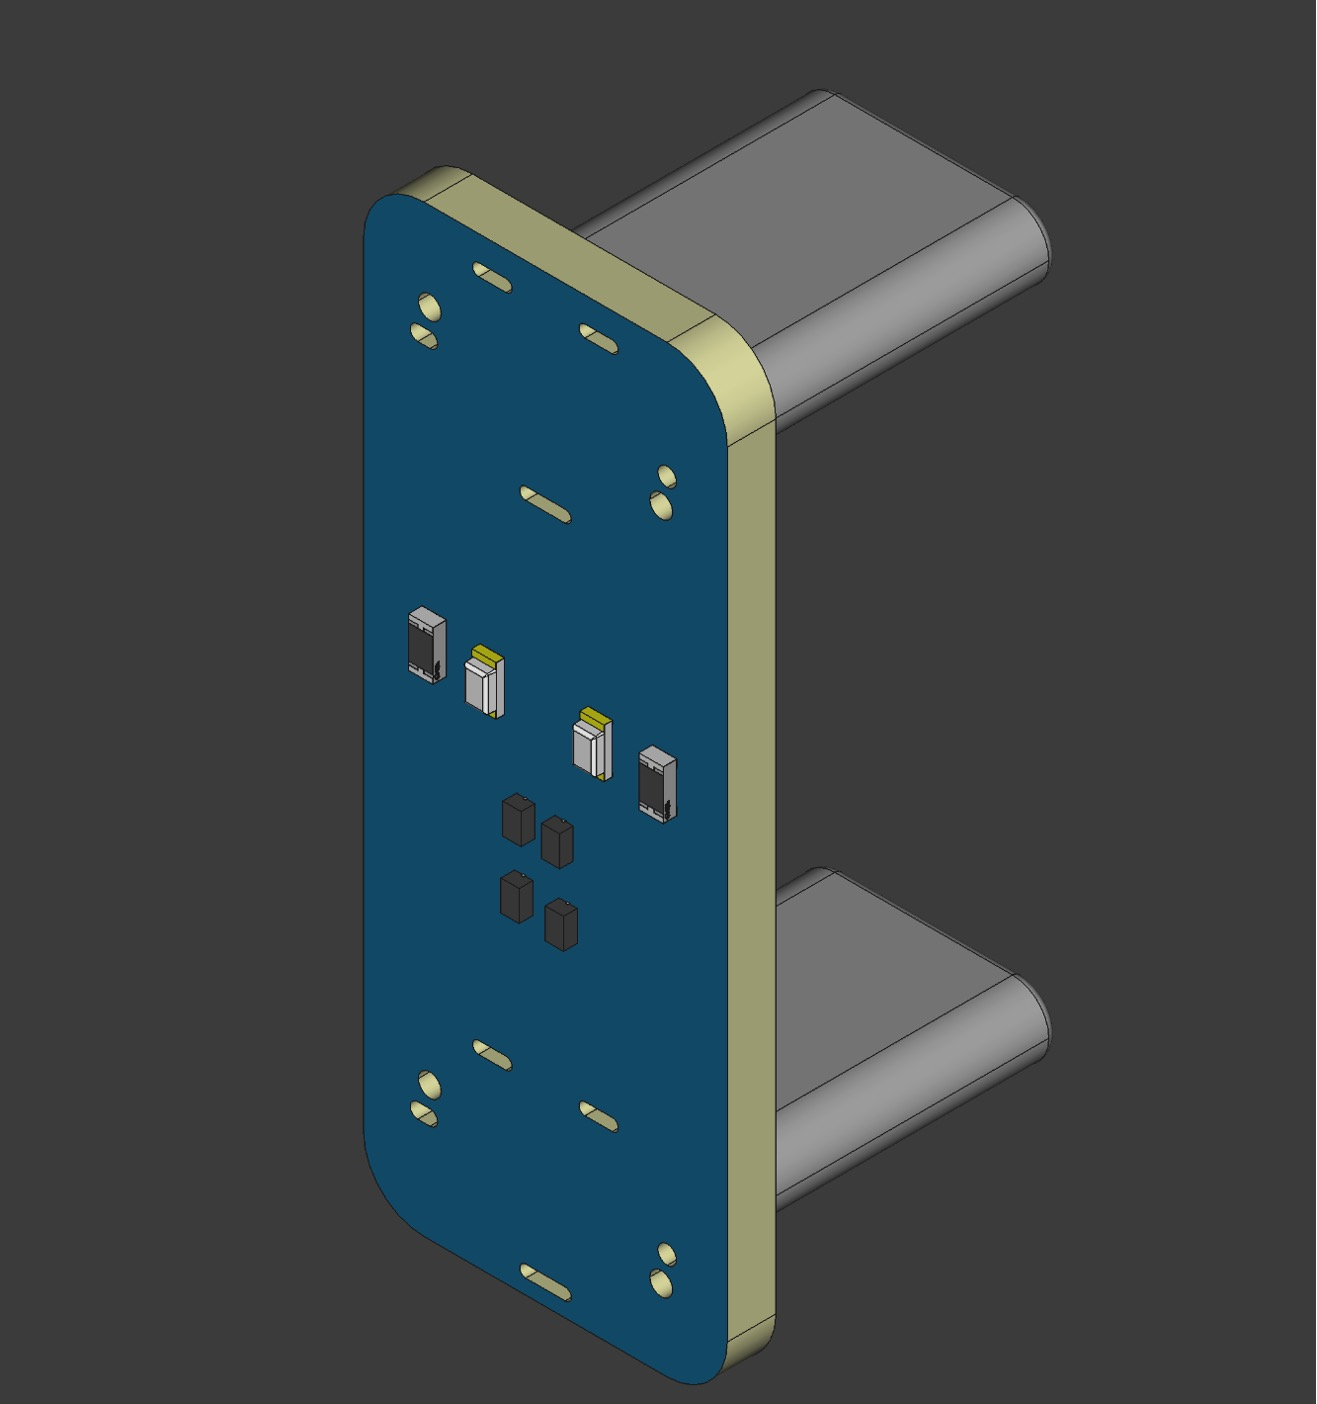
\includegraphics[width=0.9\textwidth]{images/UsbC.jpeg}
				\caption{Dimensions of Fake Usb C}
				\label{fig:UsbC}
			\end{figure}

\subsubsection{Electrical Interfaces}

\begin{figure}[H]
				\centering
				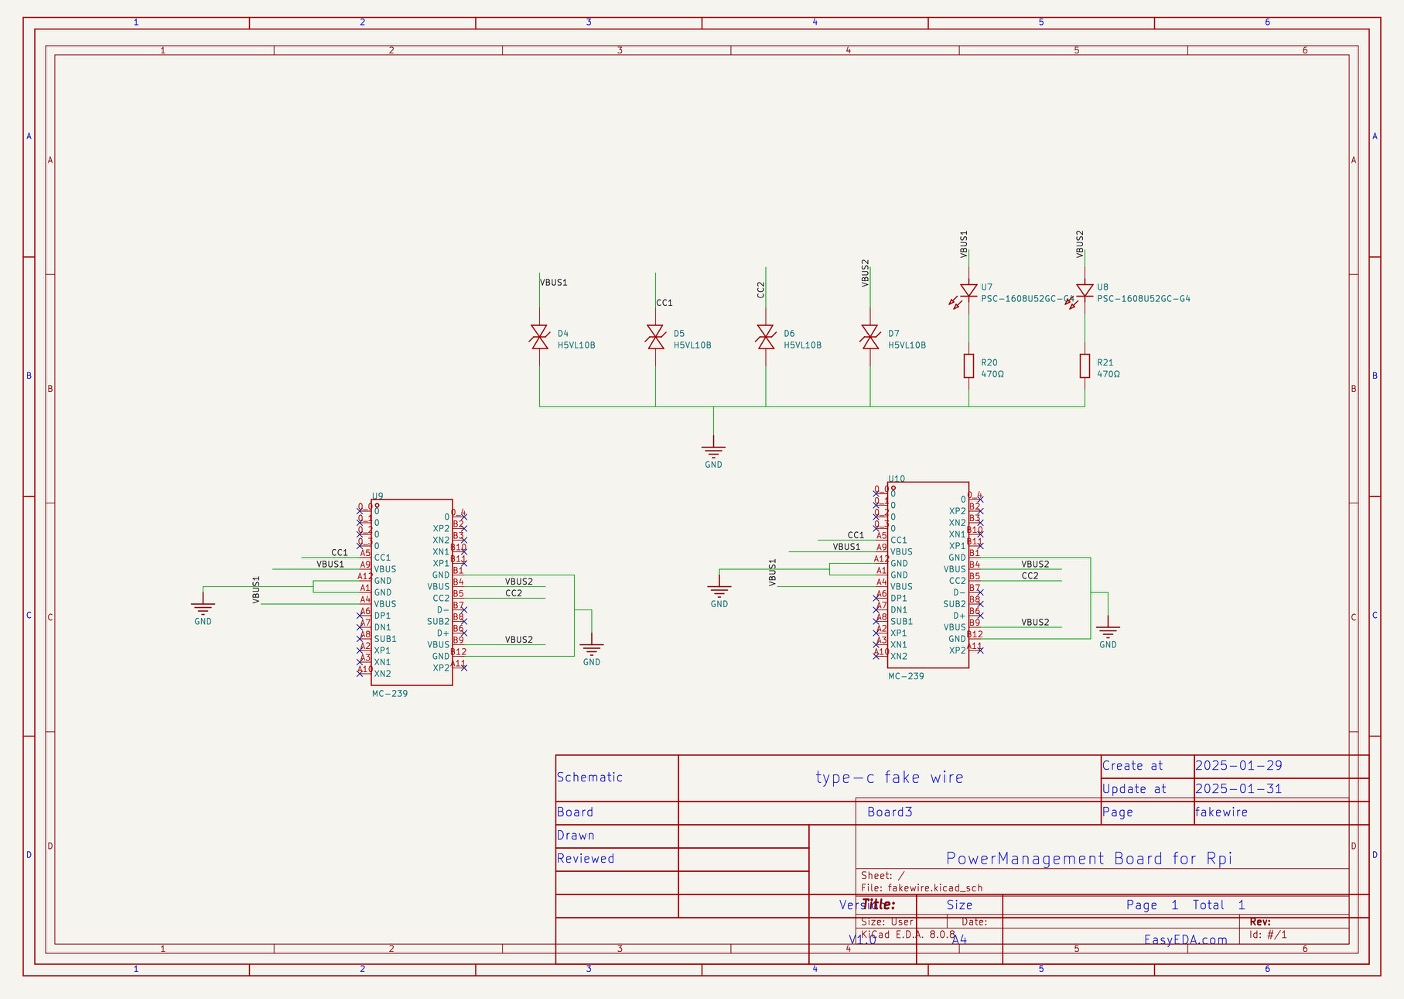
\includegraphics[width=0.9\textwidth]{images/UsbC_EI.jpeg}
				\caption{Electrical Interfaces of Fake Usb C}
				\label{fig:UsbC_EI}
			\end{figure}
			\begin{tabularx}{\textwidth}{X X}
				\toprule
				\textbf{Pin} & 	\textbf{Purpose} \\
				\midrule
					U*-VBUS & 5V, 5A power rail \\
					U*-GND & Electrical ground \\
					CC1 & Configuration Channel for PD negotiation \\
					CC2 & See above \\
				\bottomrule
			\end{tabularx}
\newpage
			\section{References }
			Raspberry Pi mechnical drawing: \\
			\url{https://pip-assets.raspberrypi.com/categories/892-raspberry-pi-5/documents/RP-008347-DS-1-raspberry-pi-5-mechanical-drawing.pdf?disposition=inline} \\
			Raspberry Pi RP1 Peripherals guide: \\
			\url{https://pip-assets.raspberrypi.com/categories/892-raspberry-pi-5/documents/RP-008370-DS-1-rp1-peripherals.pdf?disposition=inline} \\
			ToF sensors datasheet: \\
			\url{https://dl.sipeed.com/shareURL/MaixSense/MaixSense\_A010} \\
			IMU datasheet: \\
			\url{https://learn.adafruit.com/adafruit-bno055-absolute-orientation-sensor/downloads} \\
			LiDAR product page: \\
			\url{https://www.ydlidar.com/product/ydlidar-t-mini-plus} \\
			USB battery bank: \\
			\url{https://www.staples.ca/products/3119320-en-ugreen-nexode-100w-3-port-20000-mah-power-bank-portable-charger-silver} \\

\end{document}
